\documentclass[border=3pt]{standalone}
% Shared preamble for standalone figures (same fonts/colours as the paper).
\usepackage[T1]{fontenc}
\usepackage{lmodern}
\usepackage{amsmath,amssymb}
\usepackage[dvipsnames,svgnames]{xcolor}
\usepackage{tikz}
\usetikzlibrary{arrows.meta,positioning,calc,shapes.geometric,decorations.pathreplacing,shadings}
\usepackage{pgfplots}
\pgfplotsset{compat=1.18}
\usepgfplotslibrary{fillbetween}
\definecolor{pgrey}{HTML}{EEEEEE}
\definecolor{ppink}{HTML}{F8D7DA}
\definecolor{ppeach}{HTML}{FDE5C8}
\definecolor{porange}{HTML}{FBC78D}
\definecolor{pgreen}{HTML}{D4F7D4}
\definecolor{ppurple}{HTML}{EFE3F7}
\definecolor{pblue}{HTML}{DCE8F7}
\definecolor{dgreen}{HTML}{2E8B2E}
\definecolor{dpink}{HTML}{C2185B}
\definecolor{dorange}{HTML}{E07B00}
\definecolor{dblue}{HTML}{1F4E9E}
\definecolor{dpurple}{HTML}{7B3FA0}
\definecolor{gold}{HTML}{E0A800}
\tikzset{
  blk/.style={draw=black!70,rounded corners=2pt,minimum height=0.8cm,minimum width=1.9cm,
              align=center,font=\sffamily\footnotesize,inner sep=3pt},
  arr/.style={-{Stealth[length=2.2mm]},thick,black!75},
  darr/.style={-{Stealth[length=2mm]},dashed,thick},
  lbl/.style={font=\itshape\scriptsize},
}

\begin{document}
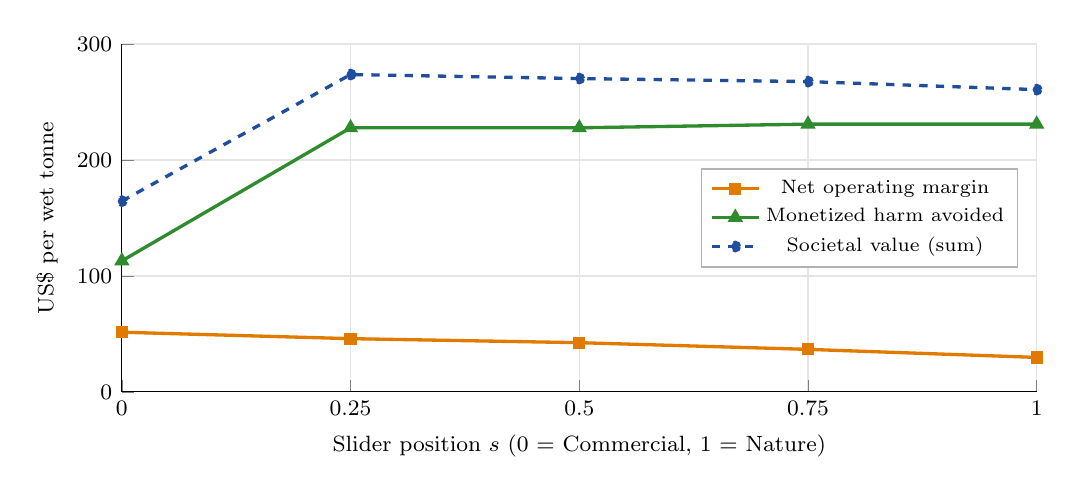
\begin{tikzpicture}
\begin{axis}[width=13.2cm, height=6cm, xmin=0, xmax=1, ymin=0, ymax=300,
  xtick={0,0.25,0.5,0.75,1}, xlabel={Slider position $s$ (0 = Commercial, 1 = Nature)},
  ylabel={US\$ per wet tonne},
  legend style={at={(0.98,0.5)},anchor=east,font=\scriptsize,draw=black!30},
  tick label style={font=\footnotesize}, label style={font=\footnotesize},
  axis x line*=bottom, axis y line*=left, grid=major, grid style={black!10}]
\addplot[dorange,very thick,mark=square*,mark size=1.6pt] coordinates {(0,51.499) (0.25,45.944) (0.5,42.475) (0.75,36.706) (1,29.769)};
\addlegendentry{Net operating margin}
\addplot[dgreen,very thick,mark=triangle*,mark size=2pt] coordinates {(0,113.008) (0.25,227.758) (0.5,227.758) (0.75,230.908) (1,230.908)};
\addlegendentry{Monetized harm avoided}
\addplot[dblue,very thick,dashed,mark=*,mark size=1.5pt] coordinates {(0,164.507) (0.25,273.702) (0.5,270.233) (0.75,267.614) (1,260.676)};
\addlegendentry{Societal value (sum)}
\end{axis}
\end{tikzpicture}
\end{document}
